
%\documentclass[11pt,a4paper,longbibliography]{article}
\documentclass[11pt,a4paper]{article} 

\setlength{\topmargin}{0cm}
\setlength{\headheight}{0.4cm}
\setlength{\headsep}{0.8cm}
\setlength{\footskip}{1cm}
\setlength{\textwidth}{17cm}
\setlength{\textheight}{25cm}
\setlength{\voffset}{-1.5cm}
\setlength{\hoffset}{-0.5cm}
\setlength{\oddsidemargin}{0cm}
\setlength{\evensidemargin}{0cm}



\usepackage{cite}


\usepackage{graphicx}				
\usepackage{pgf}

\usepackage{amsmath}				
\usepackage{amssymb}				

			
\usepackage[french]{babel}      
\usepackage[utf8]{inputenc}     		
\RequirePackage[section]{placeins}%Pour placement de section
\RequirePackage[T1]{fontenc} %Quelques lettres qui sont pas inclus dans UTF-8
\RequirePackage{mathtools} %Paquet pour des équations et symboles mathématiques
%\RequirePackage{siunitx}
\RequirePackage[justification=centering]{caption} %Pour les légendes centralisées
\RequirePackage{subcaption}

\usepackage{tabularx}				
\usepackage{psfrag}					
\usepackage{sistyle}					

\usepackage{eurosym}				

\usepackage{color}					

\definecolor{linkcolor}{rgb}{0,0,0.6}		
\usepackage[colorlinks=true,	
			pdfstartview=FitV,
			linkcolor= linkcolor,
			citecolor= linkcolor,
			urlcolor= linkcolor,
			hyperindex=true,
			hyperfigures=false]
			{hyperref}				

\usepackage{fancyhdr}				


\pagestyle{fancy}
\fancyhead[L]{\scriptsize \textsc{Génération de seconde harmonique}}
\fancyhead[R]{\scriptsize \textsc{Alexandre Fouquet}}
\fancyfoot[C]{ \thepage}


\makeatletter
\@ifpackageloaded{babel}%
        {\newcommand{\nospace}[1]{{\NoAutoSpaceBeforeFDP{}#1}}}
        {\newcommand{\nospace}[1]{#1}}
\makeatother


\newcommand{\drawat}[3]{\makebox[0pt][l]{\raisebox{#2}{\hspace*{#1}#3}}}



\begin{document}

\renewcommand{\v}[1]{\mathbf{#1}}
\newcommand{\tens}[1]{\underline{#1}}
\setlength{\parindent}{0pt}

%\pagenumbering{Alph}
\hypersetup{pageanchor=false}
\thispagestyle{empty}

\begin{@empty}

\includegraphics[height=2cm]{logoens.eps} \hfill \includegraphics[height=2cm]{logoucbl.eps} \hfill \includegraphics[height=2cm]{logounivlyon.eps}

\vspace{0.5cm}

\begin{tabularx}{\textwidth}{@{} l X l @{} }
{\sc Licence Science de la matière} 	&	& Stage 2022--2023 \\
{\it \'Ecole Normale Sup\'erieure de Lyon}		&	&  \\
{\it Universit\'e Claude Bernard Lyon I}		& 	& L3 Physique
\end{tabularx}

\begin{center}

\vspace{1.5cm}

\rule[11pt]{5cm}{0.5pt}

\textbf{\huge Génération de seconde harmonique}

\rule{5cm}{0.5pt}

\vspace{1.5cm}

\parbox{15cm}{\small
	\textbf{R\'esum\'e}: \it L'équipe de Jérôme Beugnon du groupe Gaz quantiques du Laboratoire Kastler Brossel et du Collège de France, dirigé par Jean Dalibard, manipule des gaz de Bose 2D. Le refroidissement et le piègeage des atomes nécessite de nombreux lasers, aux longeurs d'onde adaptées aux différentes transitions atomiques que l'on cherche à exploiter.
 %Les expériences de gaz d'atomes froids utilisent des lasers pour piéger les atomes qui doivent être à des longeurs d'ondes adaptées aux différentes transitions atomiques que l'on cherche à exploiter.
	L'objectif principal de mon stage a été la conception d'un laser à 532 nm (dans le vert), en utilisant non pas un cristal laser permettant d'obtenir directement un faisceau vert (par exemple \dots utilisé actuellement au laboratoire), ce type de laser étant onéreux et fragile, mais à l'aide d'une génération de fréquence double à partir d'un laser infrarouge à 1064 nm.
\vspace{0.5cm}
} 


\vspace{0.5cm}

\parbox{15cm}{
\textbf{Mots clefs} : \it Génération de seconde harmonique (SHG), niobate de lithium périodiquement polé (PPLN), fibre optique, cristaux photoniques}%TODO

\vspace{0.5cm}

\parbox{15cm}{
Stage encadr\'e par :

{\bf Jérôme \textsc{Beugnon}}

\href{mailto:beugnon@lkb.ens.fr}{\tt beugnon@lkb.ens.fr} / t\'el. (+33) 1 44 27 14 31


Laboratoire Kastler Brossel

{\it Adresse

Postale}

\url{http://adresse.web.du/laboratoire/}
} 

\vspace{0.5cm}

\includegraphics[height=5cm]{./img/logos.png}

%{\tiny \it Logos du laboratoire, de l'universit\'e d'accueil,\\ de l'organisme\ldots (\'eventuellement)}
\end{center}

\vfill
\hfill \today

\end{@empty}

\newpage

\thispagestyle{empty}
\section*{Remerciements}

Je tiens à remercier toute l'équipe Gaz quantiques du Laboratoire Kastler Brossel et du Collège de France pour son accueil chaleureux et pour m'avoir fait découvrir le monde de la recherche de l'intérieur. Je remercie tout particulièrement Franco Rabec pour avoir pris le temps de m'expliquer tous les détails de l'expérience sur laquelle il travaille et Guillaume Brochier pour sa disponibilité, son aide et ses précieux conseils, sans lesquels j'aurais été totalement perdu. Je remercie également Benjamin Huard pour m'avoir conseillé ce stage. Enfin, je remercie Jérôme Beugnon, mon maîre de stage, pour sa disponibilité, ses conseils et toutes les connaissances qu'il m'a transmises, ainsi que pour le temps qu'il m'a consacré pendant mon stage mais également en amont pour planifier mon stage et préparer tout le matériel nécessaire. 
\tableofcontents
\newpage


\setcounter{page}{1}


\setlength{\parindent}{16pt}

\section{Introduction}
Parler du labo, omniprésence des lasers (ralentissement, piègeage, excitation)

Objectif: lasers IR moins chers et plus robustes -> obtenir du vert par SHG

\section{Couplage de la fibre à cristaux/al? photoniques}
Une première partie de mon stage, indépendante de l'objectif principal d'obtenir un laser vert, a été de tester une fibre à cristaux photoniques, plus précisément un fibre de verre à c\oe ur creux LMA-PM-10 de la marque NKT Photonics. LMA signifie large (effective) mode area et donc que la fibre est faite pour des faisceaux larges, ce qui est important pour les applications avec des lasers de plusieurs dizaines de watts, car le seuil de destruction des matériaux est défini non pas par la puissance totale mais par l'intensité.

Contrairement aux fibres traditionnelles, la variation d'indice optique dans ces fibres est réalisée à l'aide d'une structure régulière de trous. En effet, l'air aillant un indice optique inférieur au matériau de la fibre, les trous permettent de réduire l'indice moyen. % TODO: corriger pour coeur creux

Il s'agit d'une fibre monomode, c'est-à-dire qu'un seul mode est sélectionné. Les fibres monomodes traditionnelles sélectionnent généralement un mode gaussien, mais la géométrie de la fibre à cristaux photoniques fait que le mode sélectionné est un mode hexagonal, comme on peut le voir figure \ref{fig:hexa}. Ce mode ne se distingue cependant que très peu d'un mode gaussien, et on ne voit la forme hexagonale que lorsque l'on sature complètement la caméra.

En particulier, afin de minimiser les pertes de puissance à travers la fibre, il faut que l'axe du faisceau incident (gaussien) coïncide avec celui de la fibre, ce qui correspond à l'ajustement de 4 paramètres (2 angles pour l'orientations et 2 coordonnées pour la position dans le plan transverse). L'ajustement aest fait à l'aide de 2 miroirs (cf schéma figure \ref{fig:couplage}). Il faut également que le faisceau ait le bon waist et qu'il soit focalisé au bon endroit. Cet ajustement se fait à l'aide d'un coupleur de fibre (60SMS-SMA-0-M5-08 de la marque Schäfter+Kirchhoff), qui est un collimateur de focale 5 mm optimisé pour le couplage de fibres. 


\begin{figure}[h]
	\centering
	\includegraphics[width=0.7\textwidth]{./img/schema couplage.png}
	\caption{Montage de la fibre à cristaux photoniques}
	\label{fig:couplage}
\end{figure}



TODO: injection en pola

\begin{figure}[h]
	\centering
	\includegraphics{./img/mode hexa.png}
	\caption{Mode hexanogal en sortie de la fibre à cristaux photoniques}
	\label{fig:hexa}
\end{figure}

\section{Principe de la génération de seconde harmonique (SHG)} %\'Etude th\'eorique de la génération de seconde harmonique (SHG)}
La propagation d'ondes électromagnétiques dans un milieu non-linéaire donne lieu à une équation d'onde avec un terme source, qui s'écrit
\[ \nabla^2 \v E_n(\v r) + \frac{\omega_n^2}{c^2}\tens\epsilon^{(1)}(\omega_n)\cdot \v E_n(\v r) = - \frac{\omega_n^2}{\epsilon_0 c^2} \v P^{NL}_n(\v r) \]
dans le domaine de Fourier en temps, avec n un indice désignant la composante spectrale (il s'agira dans notre cas de l'ordre de l'harmonique), $\tens \epsilon^{(1)}$ le tenseur de permittivité diélectrique relative associé à la partie linéaire de la polarisation et $\v P^{NL}_n$ la partie non-linéaire de la polarisation (cf annexe \ref{NL}).

En particulier, le terme d'ordre 2 $P^{(2)} = $ 

Approx paraxiale (variation en z de l'amplitude), solution (sans terme source): gaussien.

Mode q: source polarisation quadratique en l'amplitude du fondamental -> même profil transverse que $\v E_1^2 \propto \left( e^{-\left(\frac{r}{w(z)}\right)^2} \right)^2 = e^{-\left(\frac{r}{w(z)/ \sqrt 2}\right)^2}$ ce qui conduit à la supposition que le faisceau vert produit est ``gaussien'' (le profil transverse est gaussien mais la puissance varie longitudinalement) avec la même longueur de Rayleigh et un waist $\sqrt 2$ fois plus petit (ce qui est cohérent pour une longuer d'onde moitié).

On pose donc l'Ansatz suivant \[ A_2 = \frac{\mathcal A_2(z)}{1+i\zeta}e^{} \] qui correpond finalement à varier la constante dans la solution de l'équation linéaire (sans ``terme source'').

$\mathcal A_2$ vérifie alors l'équation d'évolution suivante

\begin{figure}[h]
\centering
\begin{subfigure}{0.45\textwidth}
	\includegraphics[width=\textwidth]{./img/bk-factor.pdf}
\end{subfigure}
\begin{subfigure}{0.45\textwidth}
	\includegraphics[width=\textwidth]{./img/bk-factor-cmap.pdf}
\end{subfigure}
\caption{Facteur de Boyd-Kleinman}
\label{fig:bk-factor}
\end{figure}

\section{Réalisation de la génération de seconde harmonique}
\begin{figure}[h]
	\centering
	\includegraphics{./img/schema global.png}
	\caption{Schéma du montage global}
	\label{fig:global}
\end{figure}

\begin{figure}[h]
\centering
\begin{subfigure}{0.45\textwidth}
	\includegraphics[width=\textwidth]{./img/cristal clair.jpg}
\end{subfigure}
\begin{subfigure}{0.5\textwidth}
	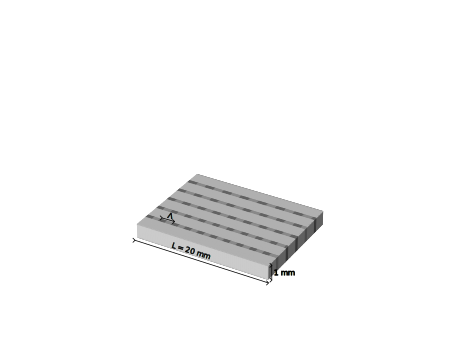
\includegraphics[width=\textwidth]{./img/cristal.png}
\end{subfigure}
\caption{Cristal doubleur de fréquence}
\label{fig:cristal}
\end{figure}



\begin{figure}[h]
    \centering
    \includegraphics{../donnees/waist faisceau incident.pdf}
    \caption{Profil du faisceau incident sur le cristal}
\end{figure}

\begin{figure}[h]
    \centering
    \includegraphics{../donnees/calib photodiode.pdf}
    \caption{Calibration de la photodiode (après glan)}
\end{figure}


\section{Étude à basse puissance}
Courbes basse puissance ($P2=f(P1^2)$ et $\alpha = f(T)$)

\begin{figure}[h]
    \centering
    \includegraphics{../donnees/conversion basse puissance 82.5 C.pdf}
    \caption{Conversion à basse puissance à 82.5°C}
\end{figure}

\begin{figure}[h]
	\centering
	\includegraphics{./img/alpha bp.pdf}
	\caption{Dépendance en température de l'efficacité de conversion}
	\label{fig:alphabp}
\end{figure}

Discussion de l'hypothèse d'égalité des longueurs de Rayleigh

\begin{figure}[h]
	\centering
	\includegraphics{./img/waist faisceau vert.pdf}
	\caption{Profil du faisceau vert généré}
	\label{fig:vert}
\end{figure}

\section{Étude à haute puissance}

\section{Conclusion}

\appendix
\section{\'Equation d'onde non-linéaire}
\label{NL}
\cite{boyd}

\section{Efficacité de conversion dans un cristal périodiquement pôlé}
Dvpt en série de Fourier de d(z)
\label{BK}



\bibliography{rapport.bib}
\bibliographystyle{unsrt}

\end{document}




